\documentclass{beamer}
%
% Choose how your presentation looks.
%
% For more themes, color themes and font themes, see:
% http://deic.uab.es/~iblanes/beamer_gallery/index_by_theme.html
%

\usefonttheme{professionalfonts}
\usefonttheme{serif}
\usepackage{fontspec}
\setmainfont{Helvetica Neue}
\setbeamerfont{note page}{family*=pplx,size=\footnotesize} % Palatino for notes

\setbeamertemplate{frametitle}
{
   \begin{centering}
   \smallskip
   \insertframetitle\smallskip\par
   \usebeamercolor[fg]{framesubtitle}\footnotesize\textit{\insertframesubtitle}\par
   \smallskip
   \end{centering}
}
\setbeamertemplate{itemize item}{--}
\setbeameroption{show notes}
\setbeamertemplate{navigation symbols}{}
\setbeamertemplate{footline}{%
    \raisebox{5pt}{\makebox[\paperwidth]{\hfill\makebox[20pt]{\color{gray}
          \scriptsize\insertframenumber}}}\hspace*{5pt}
}

\definecolor{foreground}{HTML}{D7D0CE}
\definecolor{background}{RGB}{24,24,24}
\definecolor{title}{HTML}{2380FC}
\definecolor{gray}{RGB}{155,155,155}
\definecolor{subtitle}{RGB}{102,255,204}
\definecolor{hilight}{RGB}{102,255,204}
\definecolor{vhilight}{RGB}{255,111,207}
\definecolor{alert}{HTML}{FC4438}

\setbeamercolor{titlelike}{fg=title}
\setbeamercolor{subtitle}{fg=subtitle}
\setbeamercolor{framesubtitle}{fg=subtitle}
\setbeamercolor{institute}{fg=gray}
\setbeamercolor{normal text}{fg=foreground,bg=background}
\setbeamercolor{item}{fg=foreground} % color of bullets
\setbeamercolor{subitem}{fg=gray}
\setbeamercolor{alerted text}{fg=alert}
\setbeamercolor{itemize/enumerate subbody}{fg=gray}
\setbeamertemplate{itemize subitem}{{\textendash}}
\setbeamerfont{itemize/enumerate subbody}{size=\footnotesize}
\setbeamerfont{itemize/enumerate subitem}{size=\footnotesize}
\hypersetup{colorlinks,linkcolor=foreground,urlcolor=foreground}

\let\OLDitemize\itemize
\renewcommand\itemize{\OLDitemize\addtolength{\itemsep}{15pt}}


\usepackage{pdfcomment}
\newcommand{\pdfnote}[1]{\marginnote{\pdfcomment[icon=note]{#1}}}
\newcommand{\bi}{\begin{itemize}}
\newcommand{\ei}{\end{itemize}}
\newcommand{\ig}{\includegraphics}
\newcommand{\hugeframe}[2]{
\begin{frame}[plain,c]
  \begin{center}
    \huge\textcolor{title}{#1}
    \vfill

    \normalsize #2

  \end{center}

\end{frame}}

% Fonts
\setbeamerfont{title}{size=\LARGE}


% \setbeamerfont{author}{series=\bfseries,parent=structure}
% \setbeamerfont{institute}{size=\scriptsize,series=\bfseries,parent=structure}
\setbeamerfont{date}{size=\scriptsize}


\usepackage[english]{babel}
\usepackage[utf8x]{inputenc}

\title{Big Data Analytics on Container-Orchestrated Systems}
\author{Gerard Casas Saez}
\institute{University of Colorado Boulder}
\date{July 20th}

\begin{document}

\begin{frame}
  \pdfnote{Thank  Steve Voida, Rick Han, and Tom Yeh for comming and Ken Anderson my advisor}
  \titlepage
\end{frame}

\begin{frame}{Outline}
  \tableofcontents
\end{frame}

\section{Introduction}


\begin{frame}{Introduction}

\begin{itemize}
  \item Exponential increase in data generation
  \begin{itemize}
    \item Current: 72 petabytes/month
    \item Prediction 2021: 232 petabytes/month. 
  \end{itemize}
  \item Need to scale Big Data Analytics System
  \item Keeping mantainance at low cost
  \pdfnote{322\% of increase ratio}
  \item Migrate Project EPIC architecture to new technologies
\end{itemize}

\end{frame}

% \begin{frame}{Introduction}{New technologies}

% \begin{itemize}
%   \item Microservice architectures
%   \item Container 
%   \item Container-orchestration 
%   \item Migrate existing Project EPIC current architecture to container-orchestrated system
% \end{itemize}

% \end{frame}


\section{Background}

\hugeframe{Background}

\begin{frame}{Project EPIC}

  \begin{itemize}
    \item EPIC Collect
    \item EPIC Analyze
    \item EPIC Analytics (additional machine)
  \end{itemize}
\end{frame}
\begin{frame}{Project EPIC}

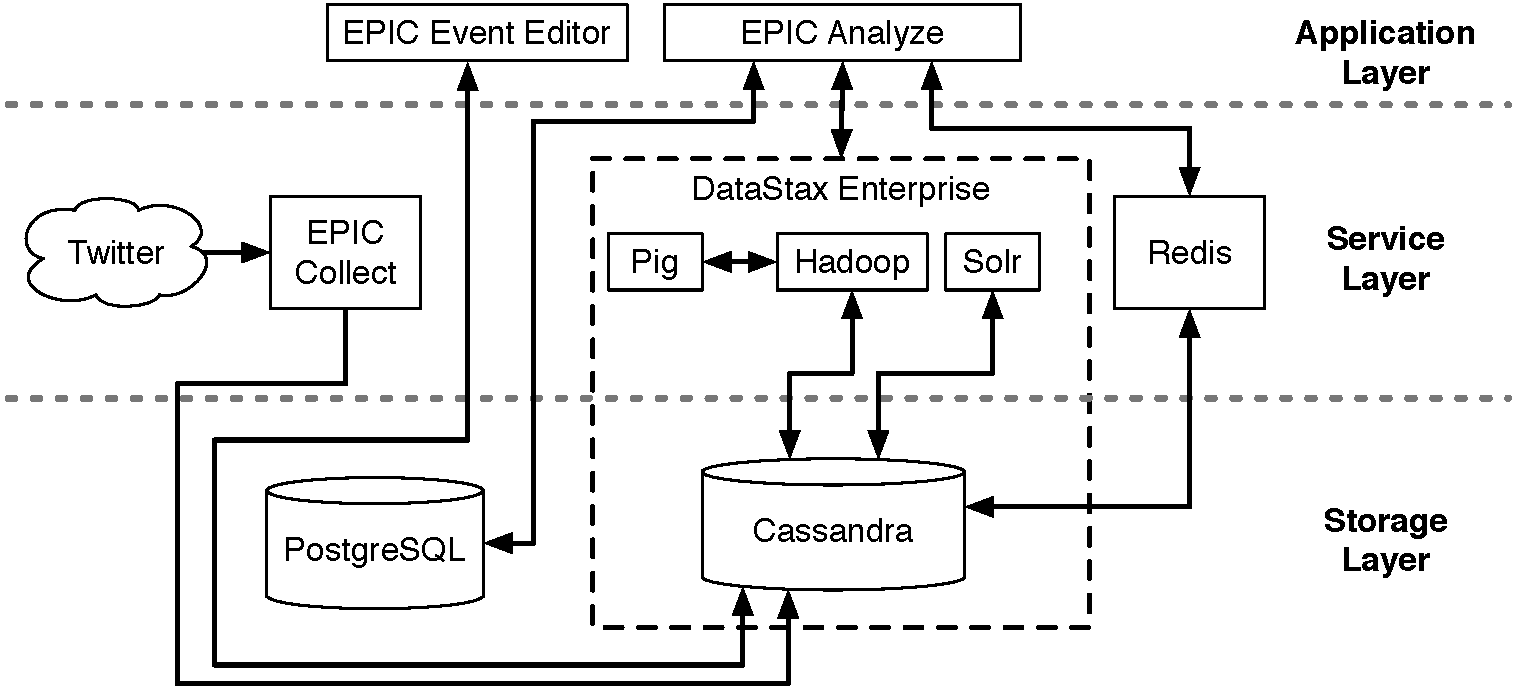
\includegraphics[width=\textwidth]{Figures/old_arch}

\end{frame}

\begin{frame}{Microservices Architecture}

  \begin{itemize}
    \item Small \& specific
    \item Highly iteractive
    \item Loosely-coupled \& highly-cohesive
    \item Independent development and scalability
  \end{itemize}

\end{frame}


\begin{frame}[plain,c]{Microservices Architecture}
  \begin{center}
    \LARGE Coreography vs Orchestration
  \end{center}

\end{frame}


\begin{frame}{Containerization}

\begin{itemize}
  \item Operating-system-level virtualization
  \item Use host machine system resources 
  \item Development microservices
  \item \textbf{Docker} most used alternative
\end{itemize}

\end{frame}

\begin{frame}{Container-orchestration systems}

\begin{itemize}
  \item Container interaction abstraction
  \pdfnote{Network configuration, interaction between containers, system updates\ldots}
  \item More mutable architectures
  \pdfnote{Allows for new possibilities for architectures}
  \item Microservices deployment
  \item Apache Mesos vs \textbf{Kubernetes}
  \item \textbf{Google Cloud}: managed Kubernetes cluster
  \pdfnote{Kubernetes is mantained by cloud native computing foundation aka Linux Foundation}
  \pdfnote{Not related to Orchestrated microservices}
\end{itemize}

\end{frame}




\section{Problem statement}
\begin{frame}{Problem statement}


\begin{enumerate}
  \item Advantages and/or limitations from the new Project EPIC infrastructure
  \begin{enumerate}
    \item More reliable?
    \item More scalable?
  \end{enumerate}
  \item Lower maintenance costs than the existing infrastructure?
  \begin{enumerate}
    \item Easier to deploy?
    \item Easier to upgrade?
    \item More resilient to failures?
  \end{enumerate}
\end{enumerate}

\end{frame}

\section{Approach}
\hugeframe{Approach}{}

\begin{frame}{Features}

\begin{itemize}
  \item Event management
  \item Real-time collection of streaming Twitter data
  \item Real-time classification of incoming tweets
  \item Data Analysis
\end{itemize}

\end{frame}

\begin{frame}{Custom components}

\begin{itemize}
  \item \textbf{Event Manager:} CRUD UI for events

  \item \textbf{Infrastructure Controller:} Changes infrastructure on demmand

  \item \textbf{Twitter Tracker:} Twitter streaming client

  \item \textbf{Twitter Normalizer:} JSON to cassandra row
\end{itemize}

\end{frame}

\begin{frame}{Architecture}

\begin{figure}
\colorbox{white}{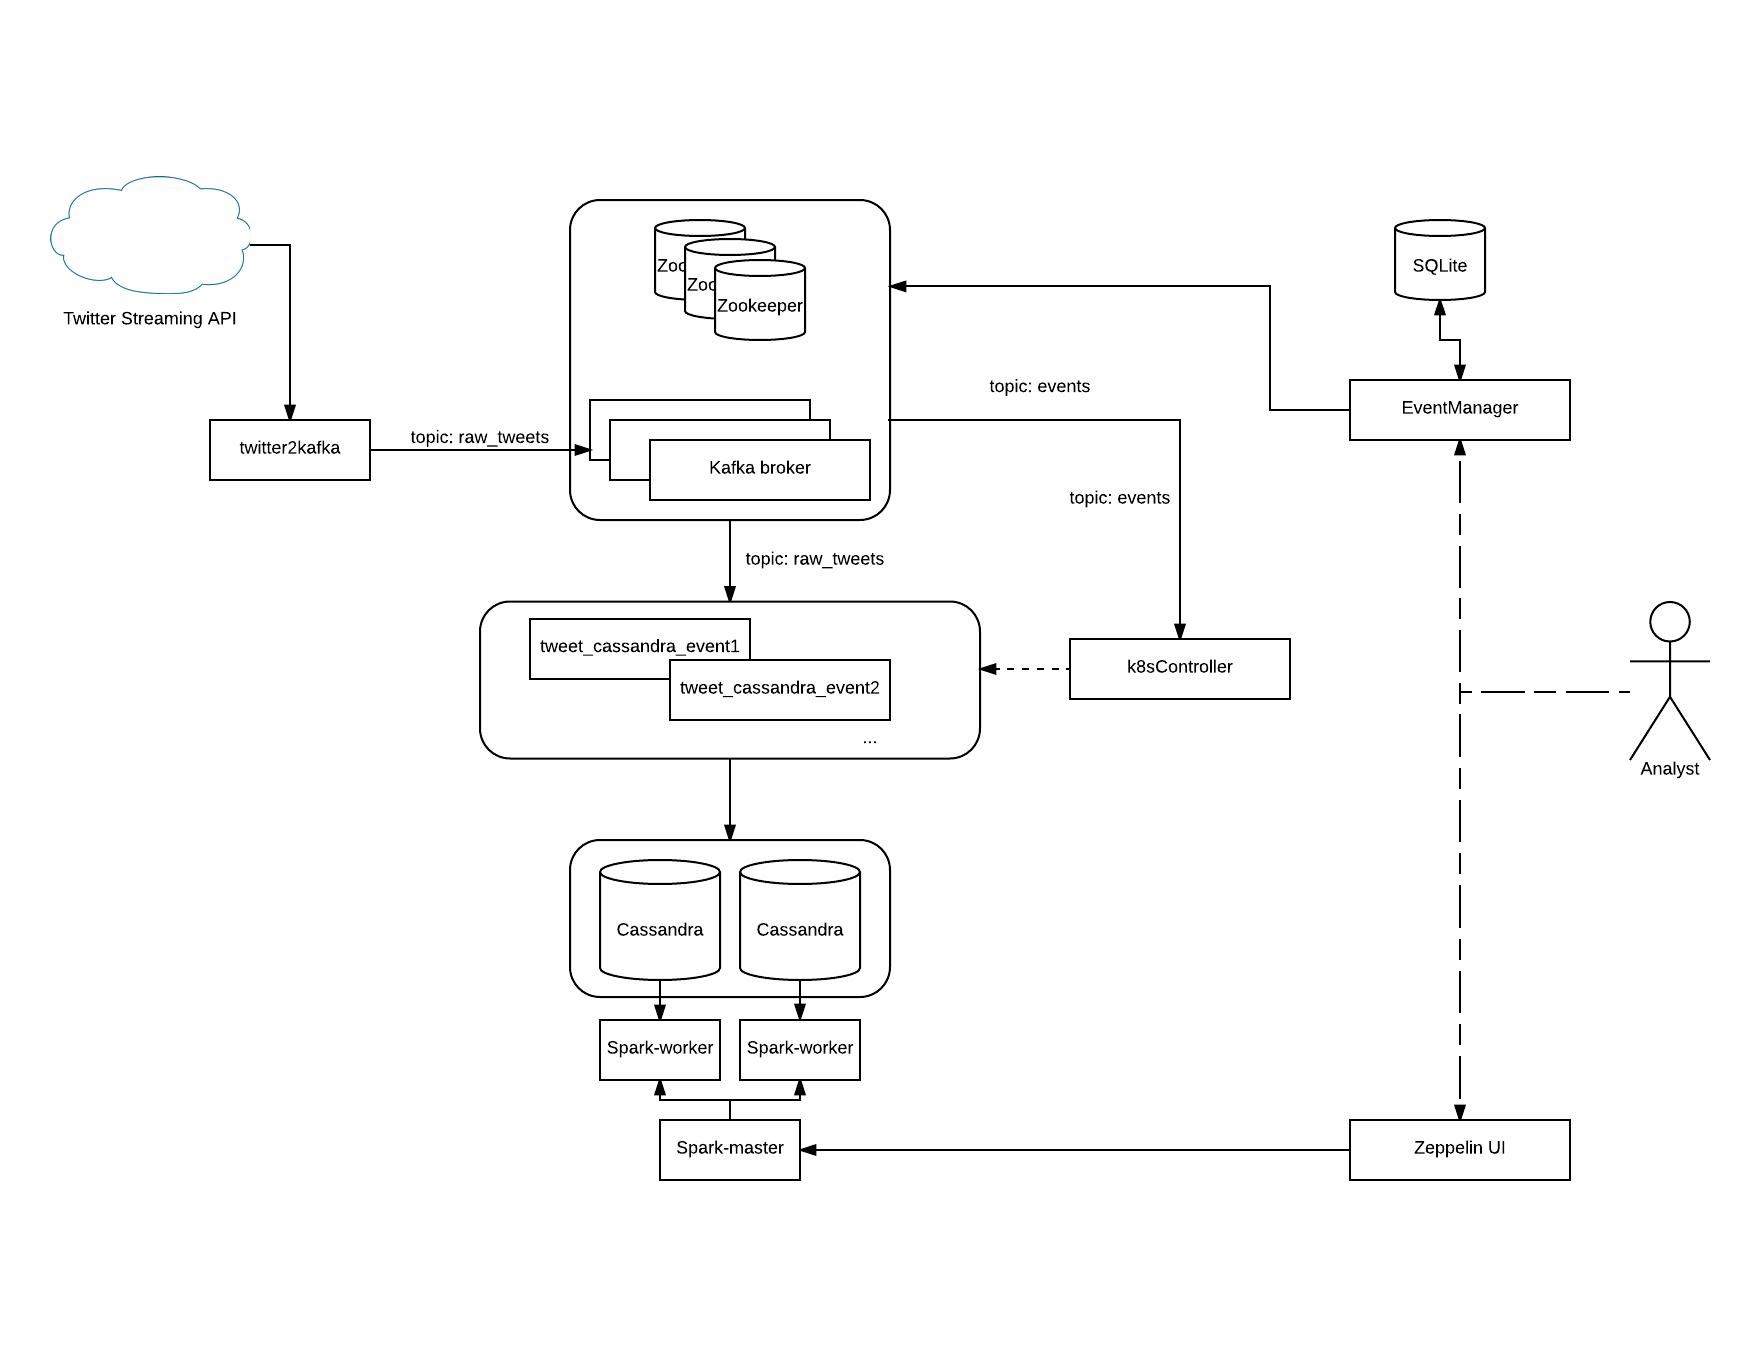
\includegraphics[width=\textwidth]{Figures/SysArch}}
\end{figure}

\end{frame}

\section{Implementation}
\hugeframe{Implementation}{}


\hugeframe{Let's track an event...}{\href{http://epic.gerard.space}{Event Manager UI}}
\hugeframe{...and analyze it!}{\href{http://epic.gerard.space/zeppelin/}{Zeppelin Notebook}}



\section{Questions?}
\hugeframe{Questions?}{}


% Commands to include a figure:
%\begin{figure}
%\includegraphics[width=\textwidth]{your-figure's-file-name}
%\caption{\label{fig:your-figure}Caption goes here.}
%\end{figure}

% \begin{table}
% \centering
% \begin{tabular}{l|r}
% Item & Quantity \\\hline
% Widgets & 42 \\
% Gadgets & 13
% \end{tabular}
% \caption{\label{tab:widgets}An example table.}
% \end{table}

% \end{frame}


\end{document}
